\documentclass[a4paper,12pt]{article}
\usepackage{graphicx}
\usepackage[UTF8]{ctex}
\usepackage{fontspec}
\usepackage{booktabs}
\usepackage{float}%浮动体
\usepackage{amsmath,amssymb}
\usepackage{fancyhdr}
%\usepackage{xcolor}
\usepackage{colortbl}
\usepackage{geometry}
\geometry{top=2cm,bottom=2cm,left=1cm,right=1cm}
\begin{document}
	\begin{figure}[H]
	\begin{center}
		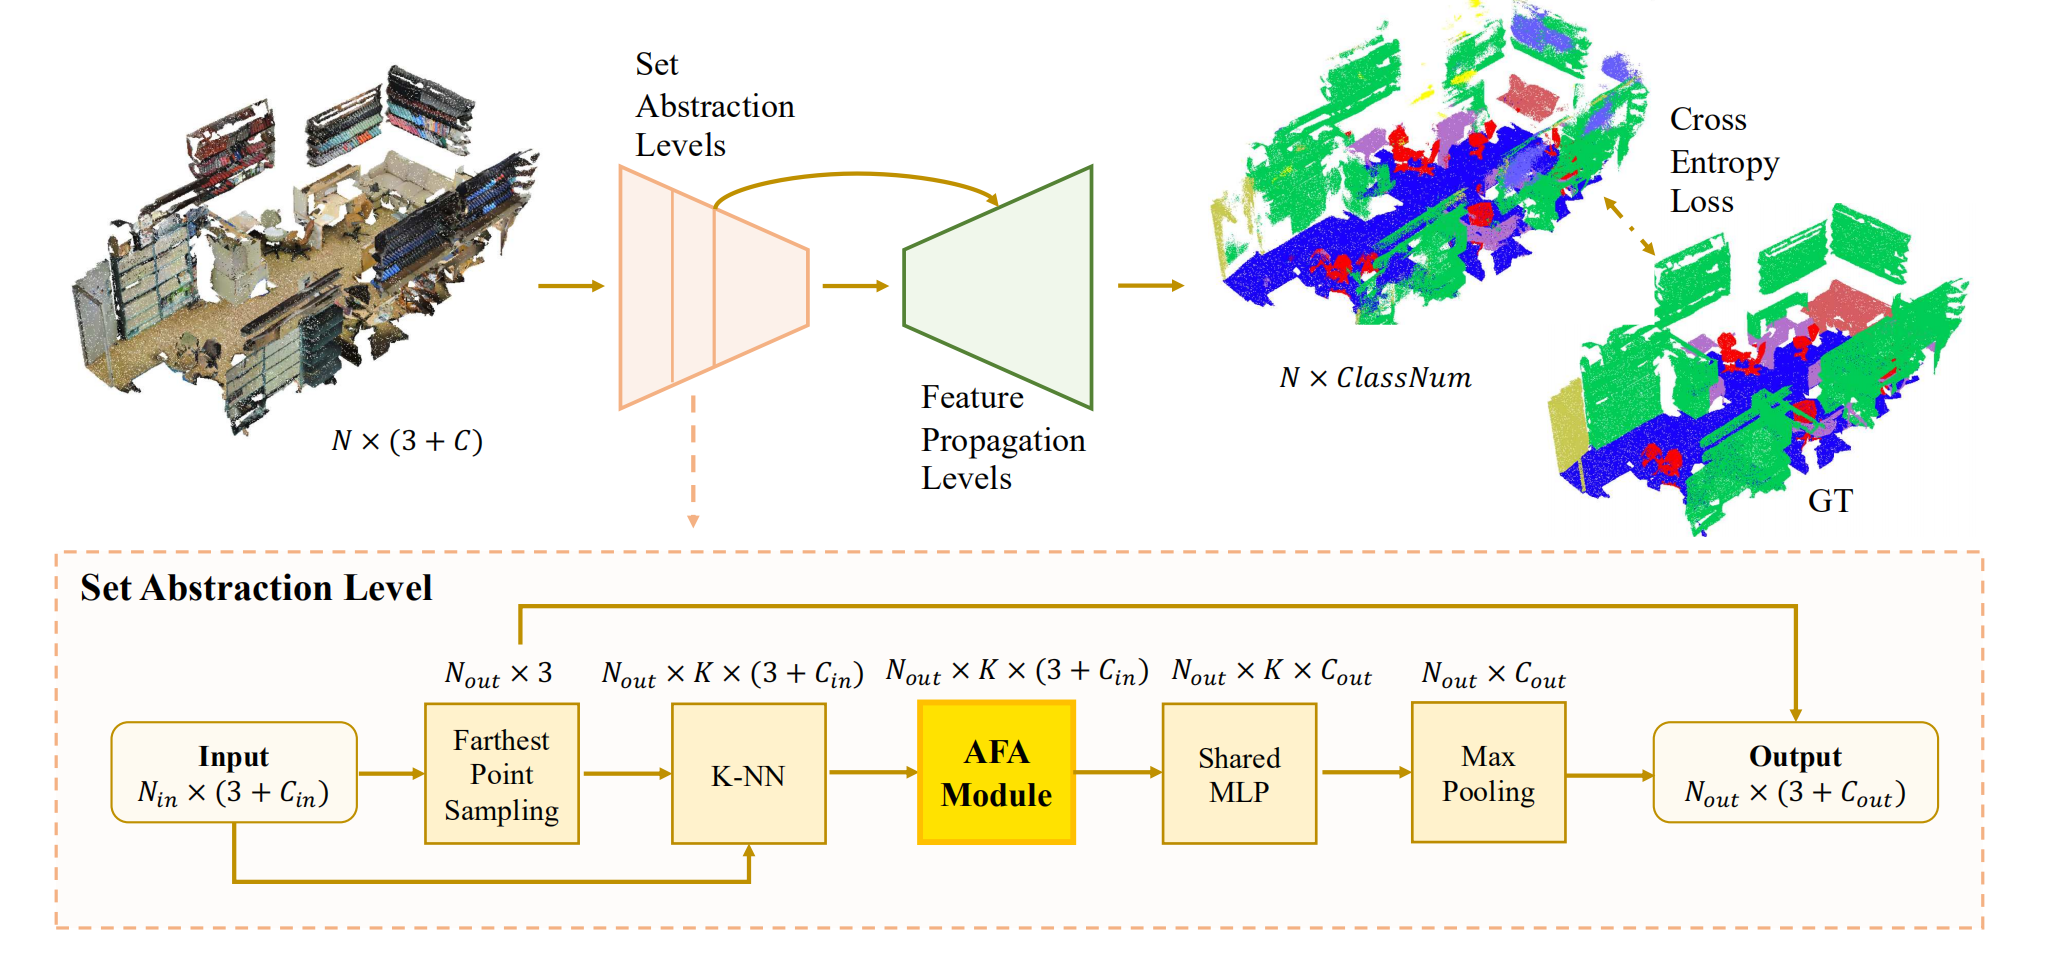
\includegraphics[width=0.9\textwidth]{img/PointWeb.png} 
		\caption{PointWeb}
	\end{center}
\end{figure}

	\begin{figure}[H]
		\begin{center}
			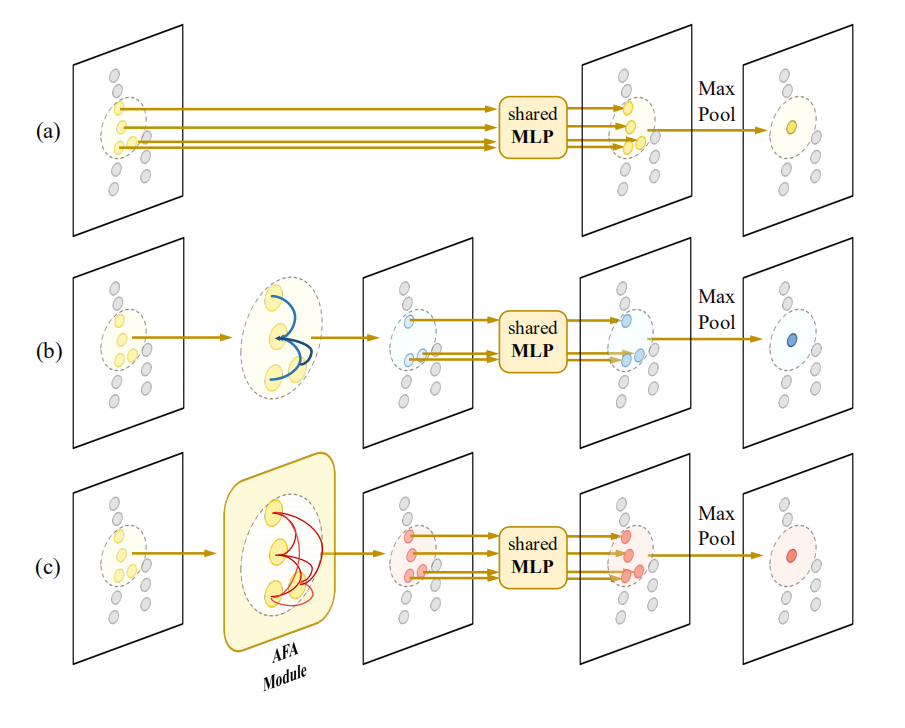
\includegraphics[width=0.9\textwidth]{img/PointNet++_PointWeb_DGCNN.png} 
			\caption{PointNet++\_PointWeb\_DGCNN}
		\end{center}
	\end{figure}





\textbf{分析}:
\begin{itemize}
	\item PointNet++提取特征的方法不涉及局部邻域点之间的区域信息交换。
	\item 将DGCNN以$x_i$为中心的图变成一张每个点都互联的web
	\item 总体的处理结构与PointNet++类似,就是特征提取部分有所不同
\end{itemize}
$$
\begin{aligned}
	&F_{i}^{\prime}=F_{i}+\Delta F_{i}\\
	&\Delta F_{i}=f_{\operatorname{mod}}\left(F_{i}, \mathbb{F}\right), \forall F_{i} \in \mathbb{F}\\
	&f_{m o d}\left(F_{i}, \mathbb{F}\right)=\sum_{j=1}^{M} f_{i m p}\left(F_{i}, F_{j}\right) \cdot f_{\text {rel }}\left(F_{i}, F_{j}\right)\\
	&\operatorname{f_{imp}}\left(F_{i}, F_{j}\right)=\operatorname{MLP}\left(g\left(F_{i}, F_{j}\right)\right) \text {. }\\
	&g\left(F_{i}, F_{j}\right)=F_{i}-F_{j}\\
	&f_{rel}\left(F_{i}, F_{j}\right)= \begin{cases}F_{i}-F_{j} & \text {, if } i \neq j \\ F_{i} \quad, & \text { if } i=j\end{cases}\\
	&F_{i}^{\prime}=\alpha_{i}^{(i)} \cdot F_{i}+\sum_{j=1, j \neq i}^{M} \alpha_{j}^{(i)}\left(F_{j}-F_{i}\right)\\
	&\alpha_{j}^{(i)}= \begin{cases}-f_{i m p}\left(F_{i}, F_{j}\right) & \text { if } i \neq j \\ 1+\operatorname{f_{i m p}}\left(F_{i}, F_{i}\right) & \text { of } i=j\end{cases}
\end{aligned}
$$

\paragraph{分类任务}
同PointNet++
\paragraph{语义分割} 同PointNet++

\end{document}